%!TeX root=MemoriaTFG.tex

\chapter{User guide}\label{ann:user-guide}

This annex gives a practical overview of how Wave Launcher is used. Chapter~\ref{chap:validation} describes the environments, procedure and results used to validate the same operations.

\section{Initial configuration}

On the first launch, the user opens Settings and goes to the Java area. Mojang and Eclipse Adoptium are available as suppliers. The selected release is installed in Wave Launcher's application-data directory, which keeps it separate from system-wide Java installations.

\begin{figure}[htbp]
  \centering
  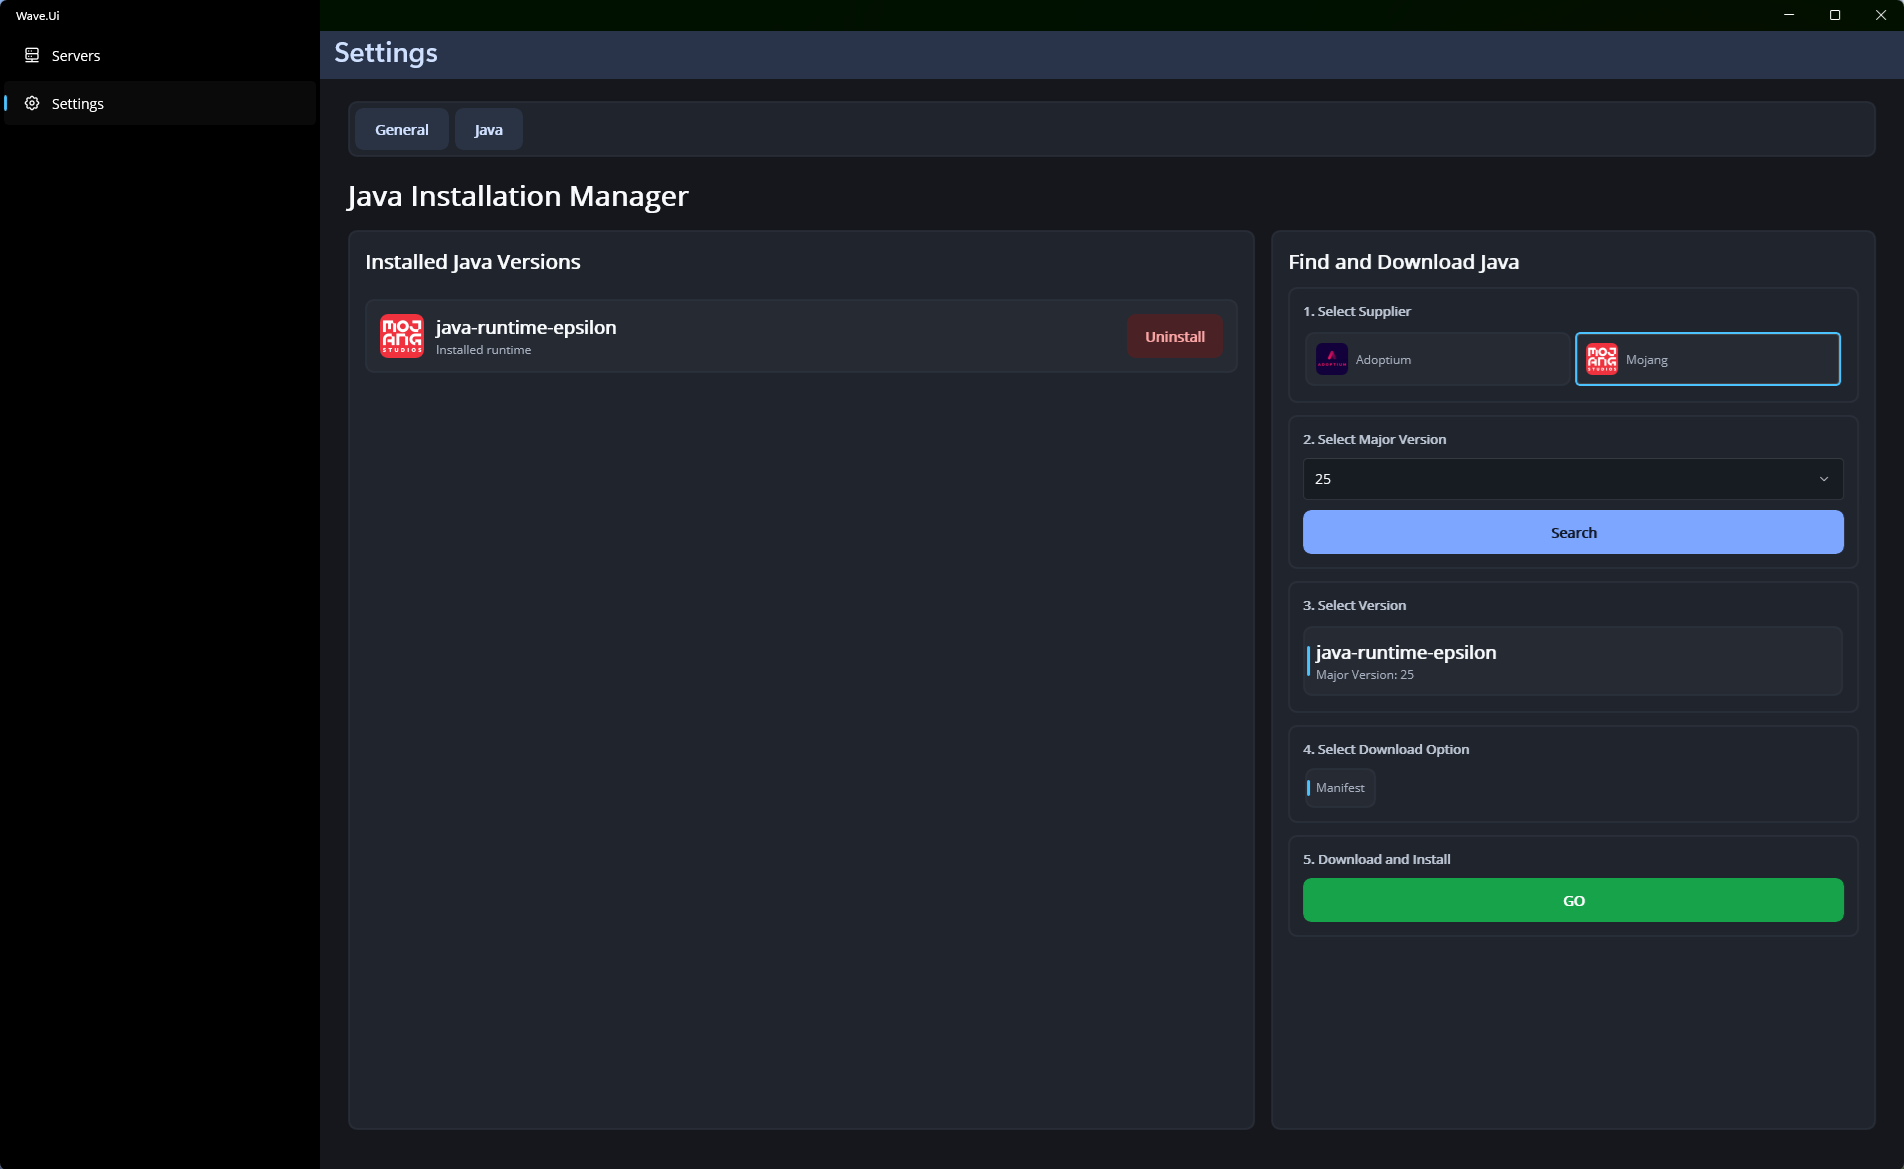
\includegraphics[width=\textwidth,height=0.72\textheight,keepaspectratio]{JavaSettings.png}
  \caption{Java runtime configuration.}
  \label{fig:guide-java-settings}
\end{figure}

To use CurseForge, the user must also enter an API token in the general application settings. Modrinth does not require this token.

\begin{figure}[htbp]
  \centering
  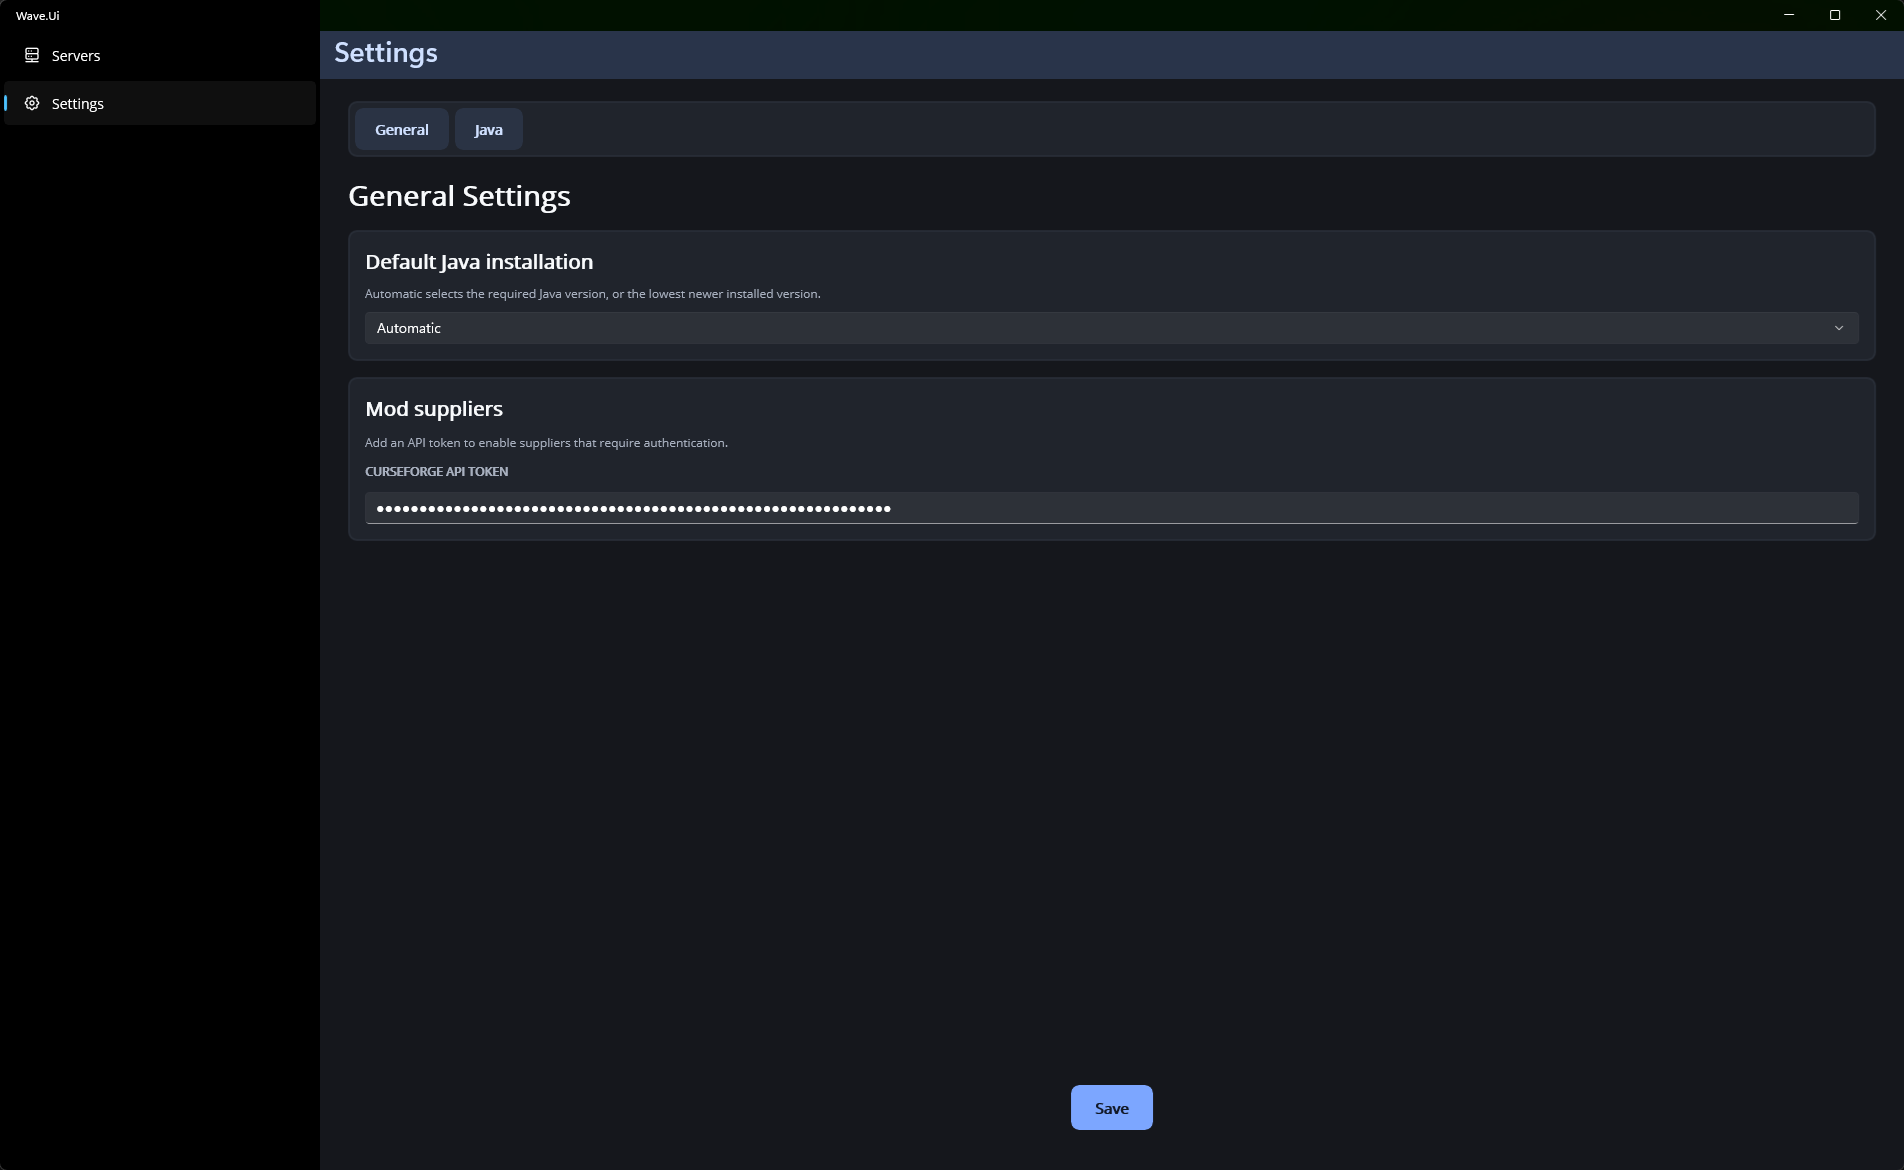
\includegraphics[width=\textwidth,height=0.72\textheight,keepaspectratio]{AppSettings.png}
  \caption{Application and provider settings.}
  \label{fig:guide-app-settings}
\end{figure}

\section{Creating a server}

From the Servers page, the user creates a new instance and supplies a name. An icon can be selected, after which the application stores a normalized copy. The Minecraft release and Java runtime are chosen from the presented lists. Snapshot visibility can be enabled when an unstable Minecraft release is required.

\begin{figure}[htbp]
  \centering
  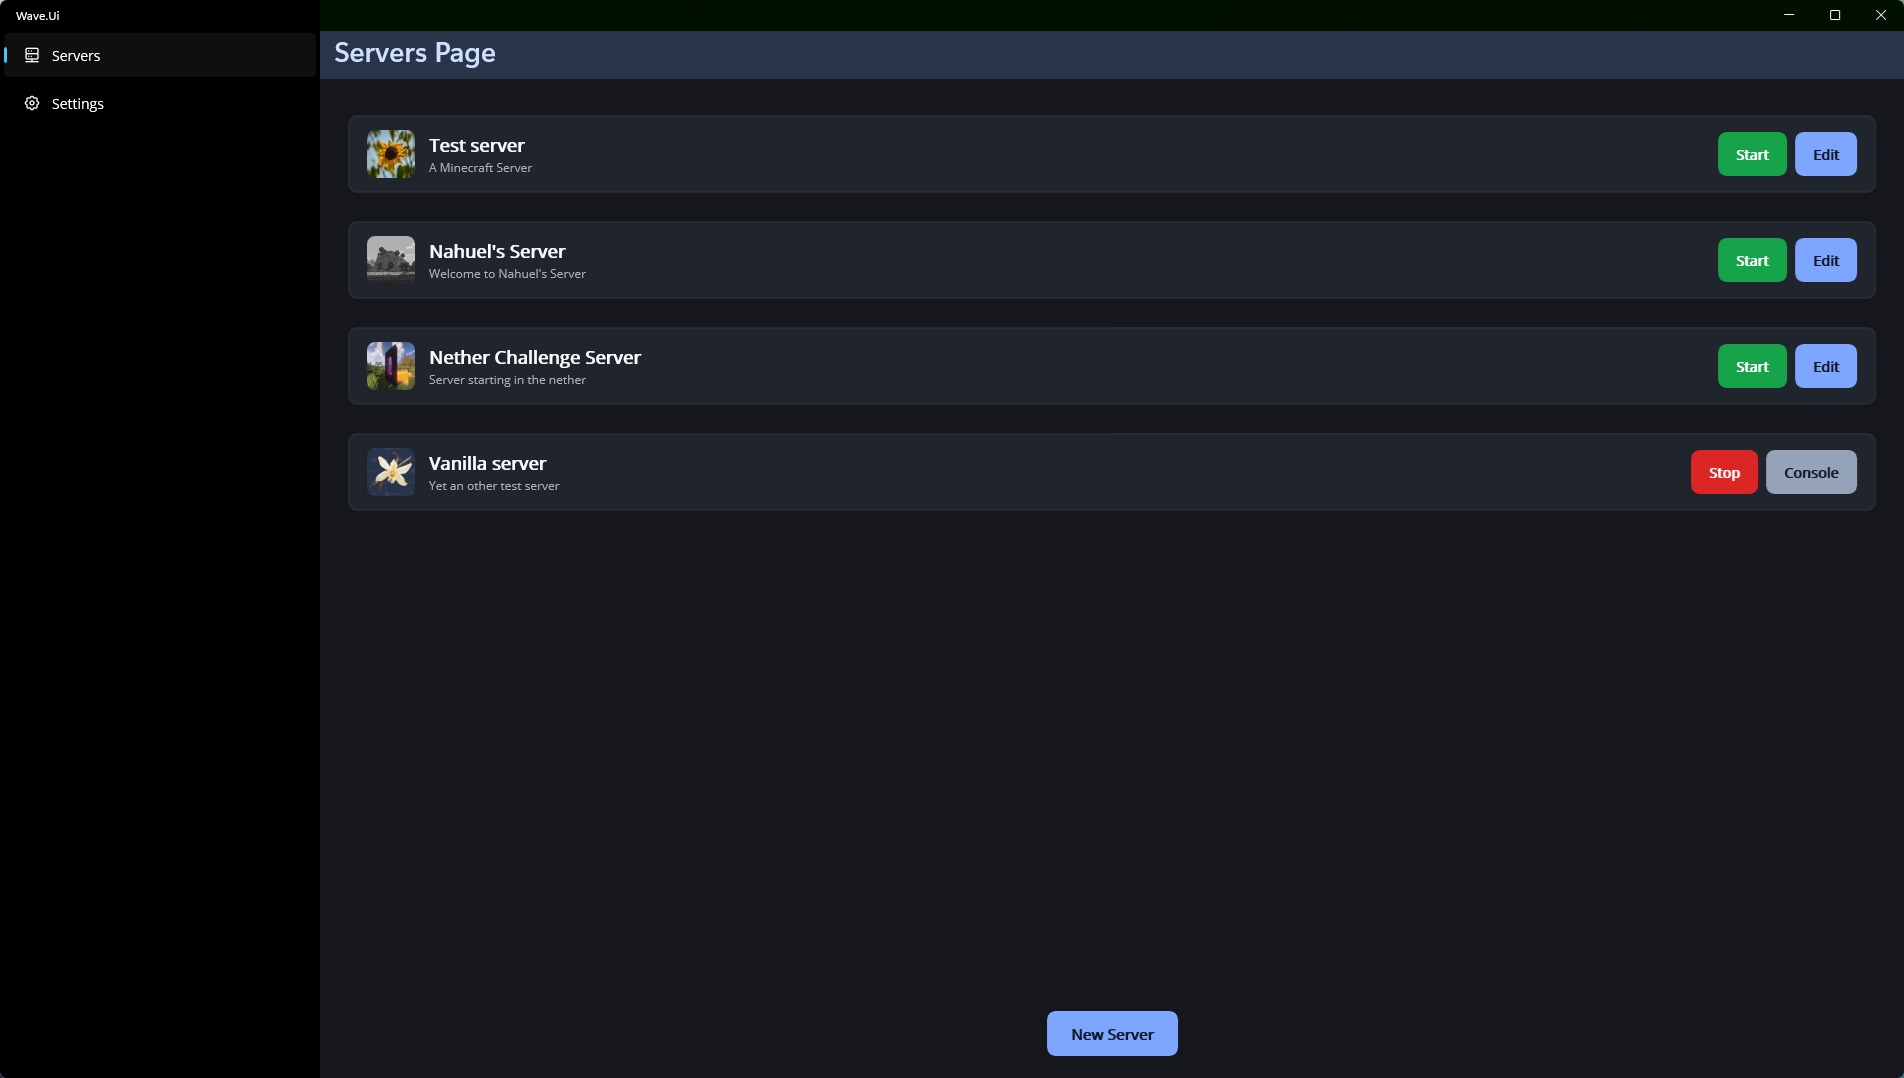
\includegraphics[width=\textwidth,height=0.72\textheight,keepaspectratio]{ServersPage.png}
  \caption{Server list and new-server action.}
  \label{fig:guide-servers-page}
\end{figure}

\begin{figure}[htbp]
  \centering
  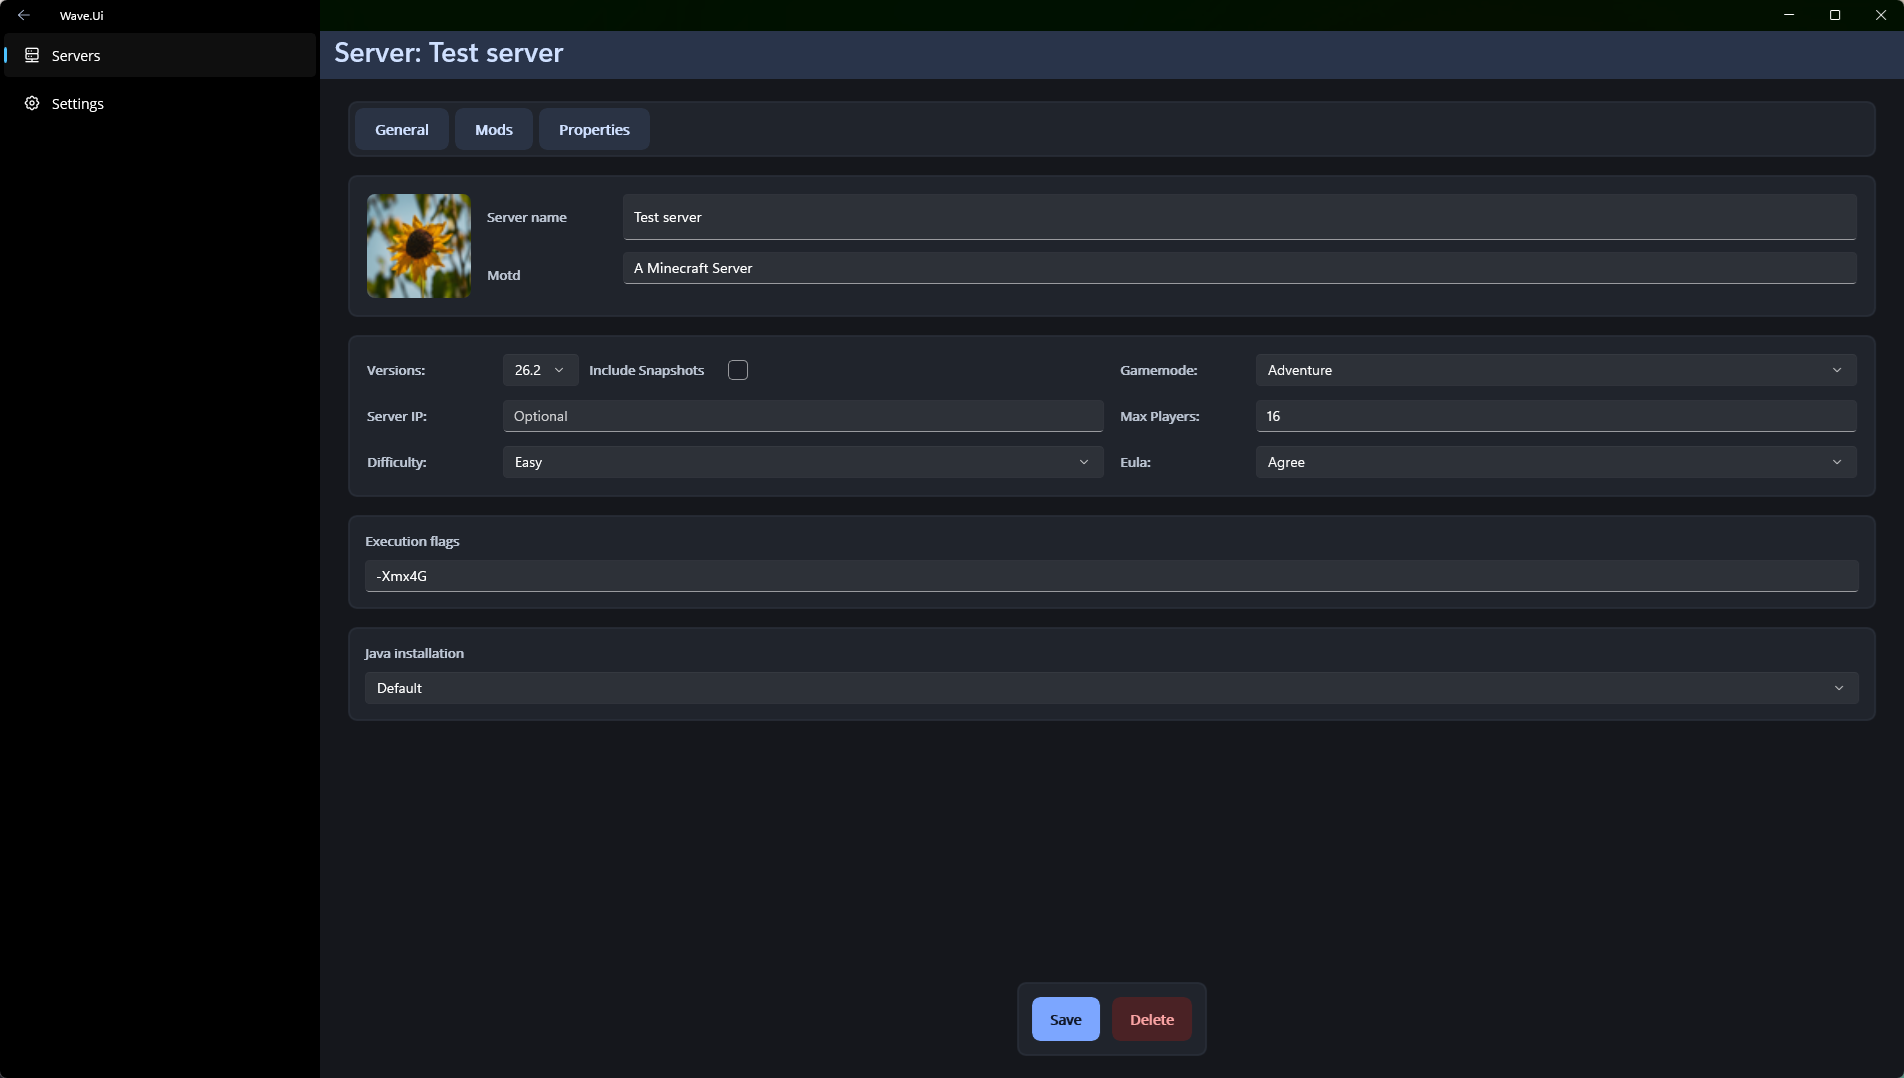
\includegraphics[width=\textwidth,height=0.72\textheight,keepaspectratio]{ServerConfigurationPage.png}
  \caption{General configuration for a new server.}
  \label{fig:guide-server-configuration}
\end{figure}

The General area contains launch options and EULA acceptance. The Properties area exposes the Minecraft configuration definitions through typed controls. If a modded server is desired, Forge or Fabric and one of its compatible releases is selected. Mods can then be searched from the Mods area. Submitting the form downloads and constructs the complete server directory.

\begin{figure}[htbp]
  \centering
  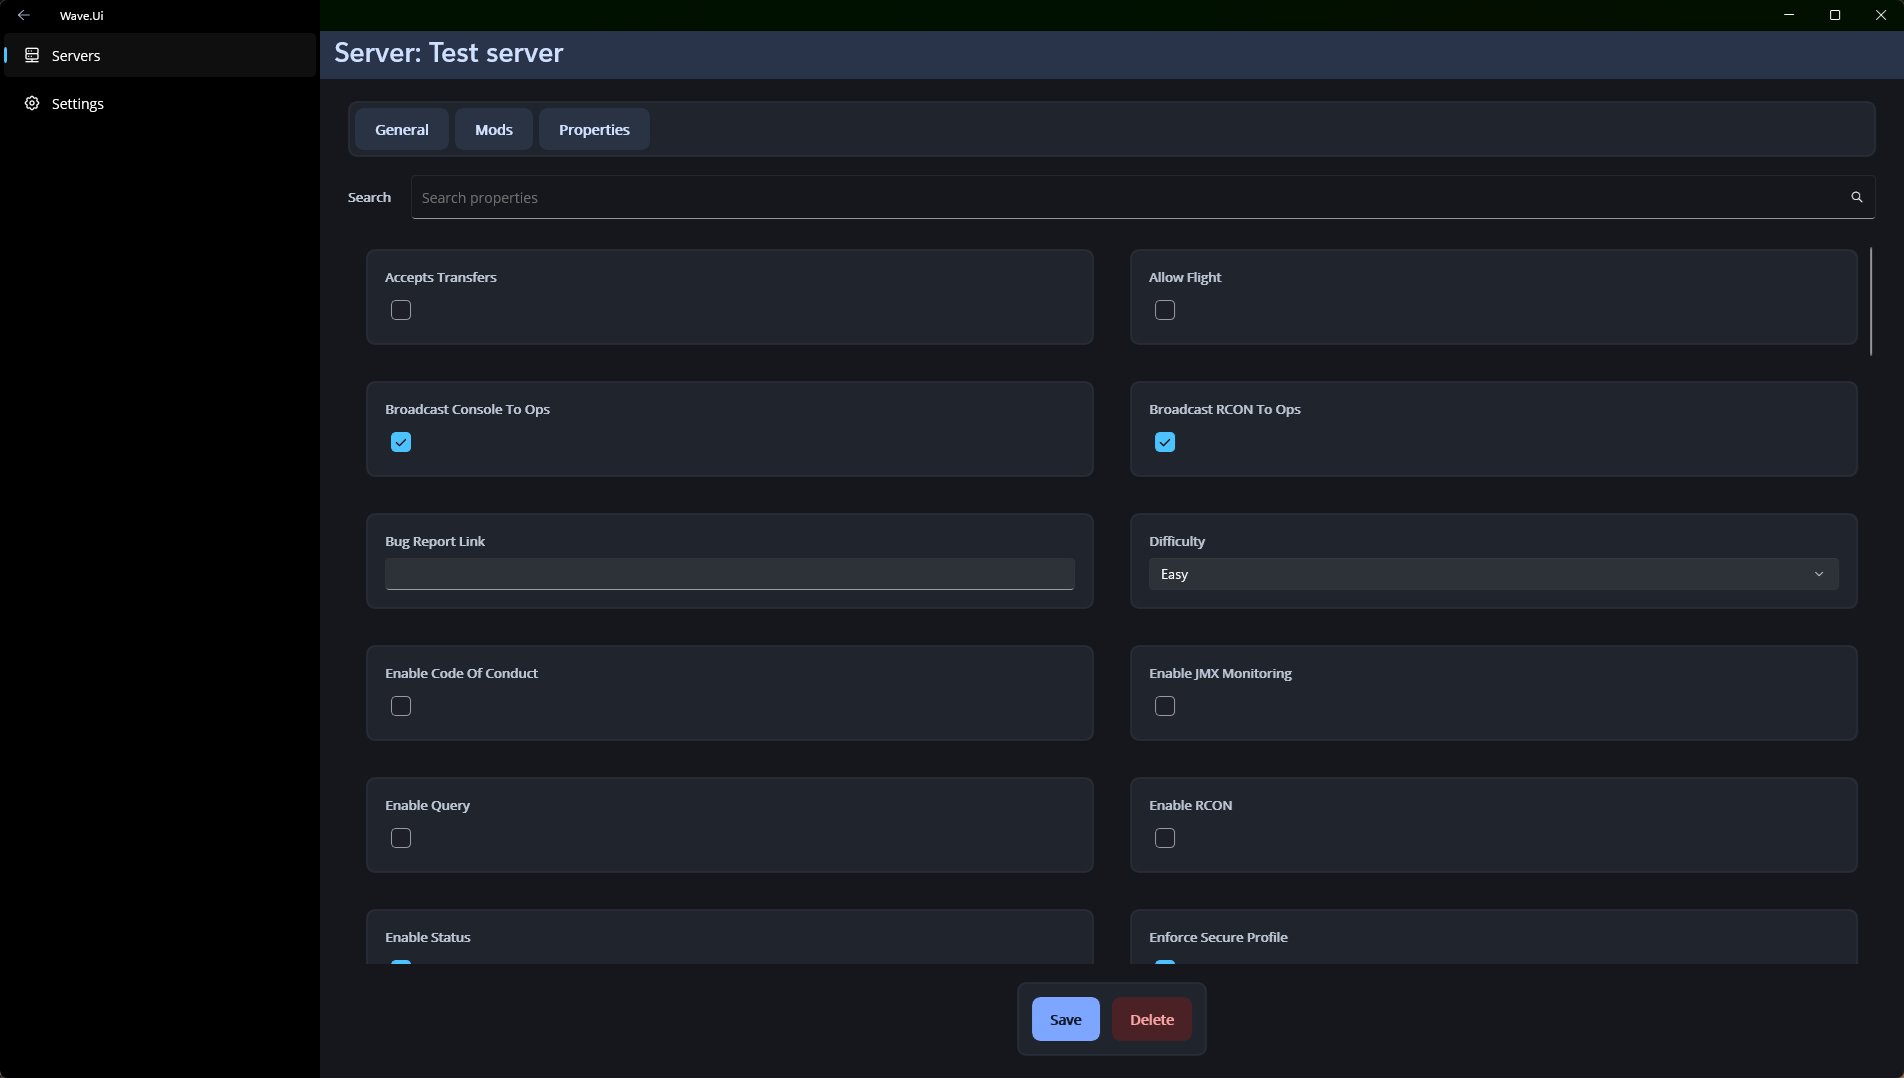
\includegraphics[width=\textwidth,height=0.72\textheight,keepaspectratio]{ServerPropertiesPage.png}
  \caption{Minecraft server-properties configuration.}
  \label{fig:guide-server-properties}
\end{figure}

\begin{figure}[htbp]
  \centering
  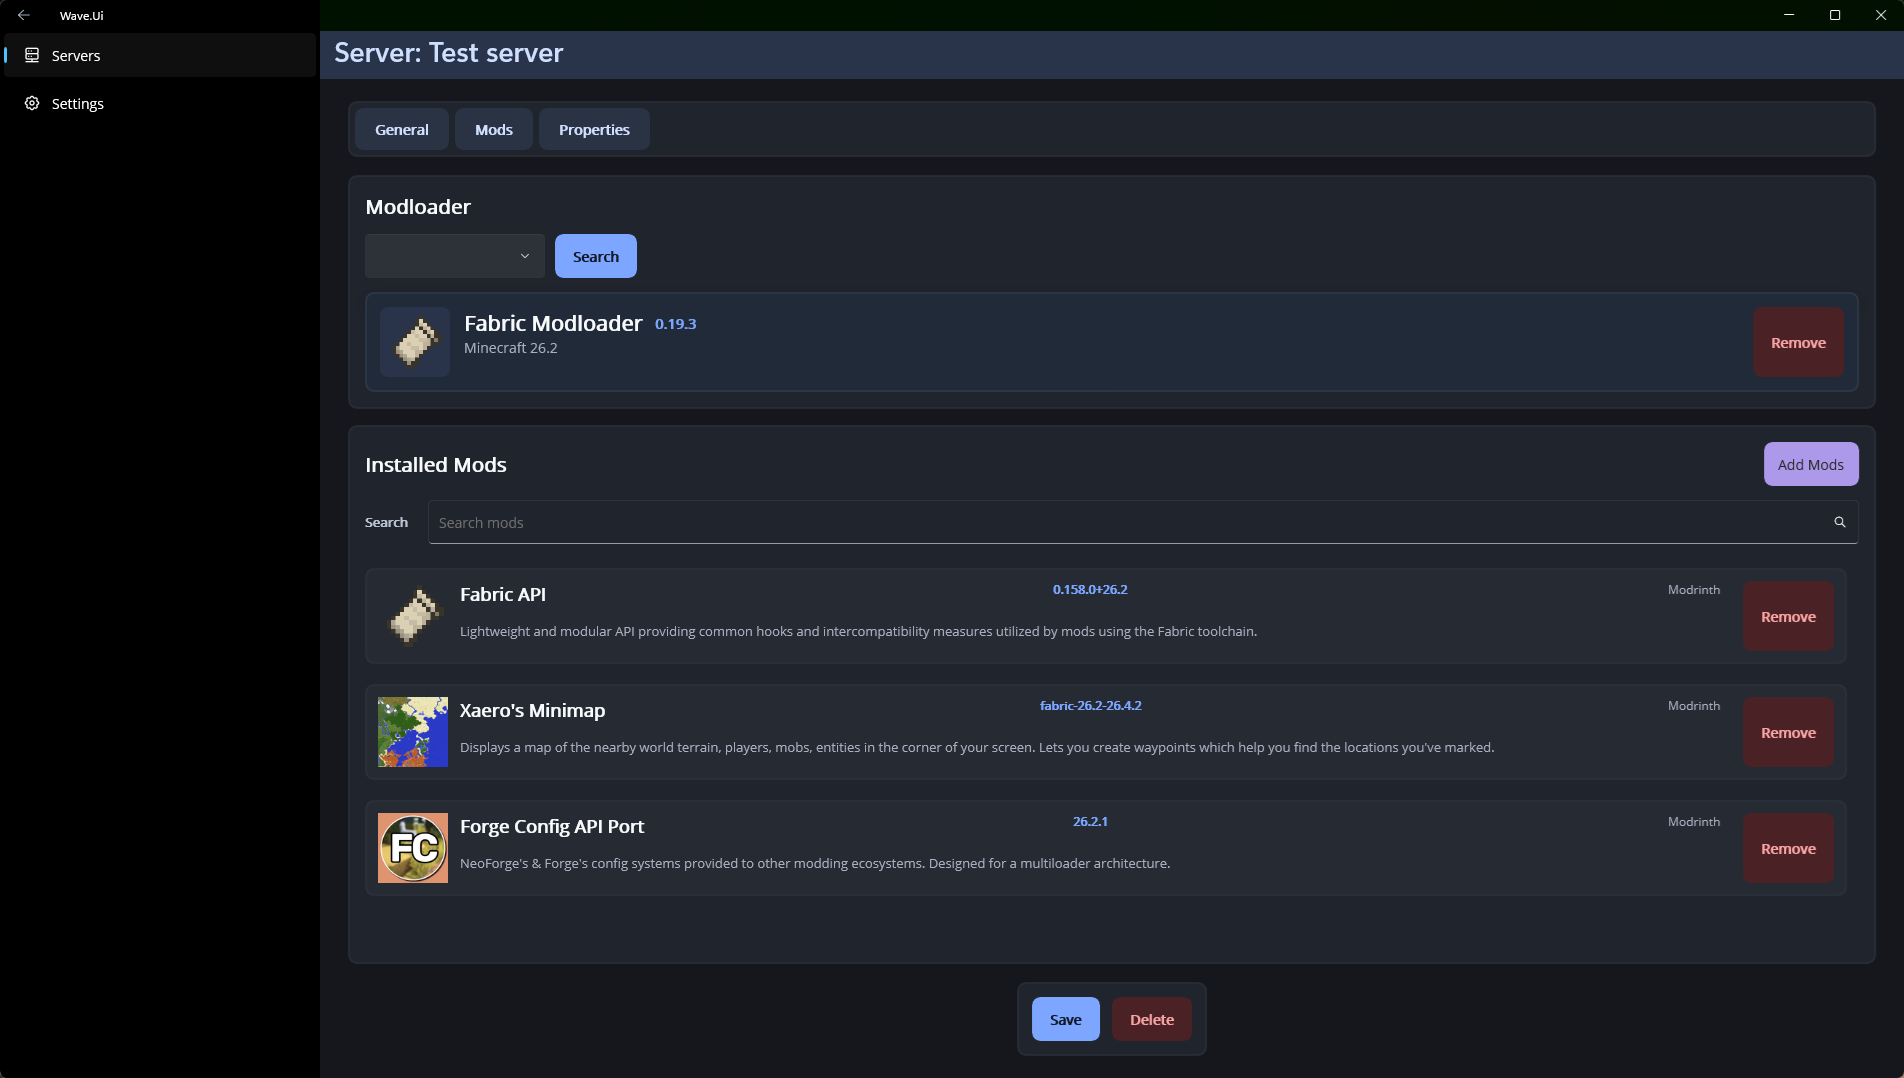
\includegraphics[width=\textwidth,height=0.72\textheight,keepaspectratio]{ServerModsPage.png}
  \caption{Loader and installed-mod configuration.}
  \label{fig:guide-server-mods}
\end{figure}

\section{Editing and migrating}

Selecting an existing card opens the same editor with stored values. Ordinary settings can be changed directly. A Minecraft or loader change may require replacement or removal of related components. Before applying the edit, the changes popup summarizes these consequences. After confirmation, Wave Launcher downloads compatible artifacts and reports mods that were required, incompatible, unavailable or failed.

\begin{figure}[htbp]
  \centering
  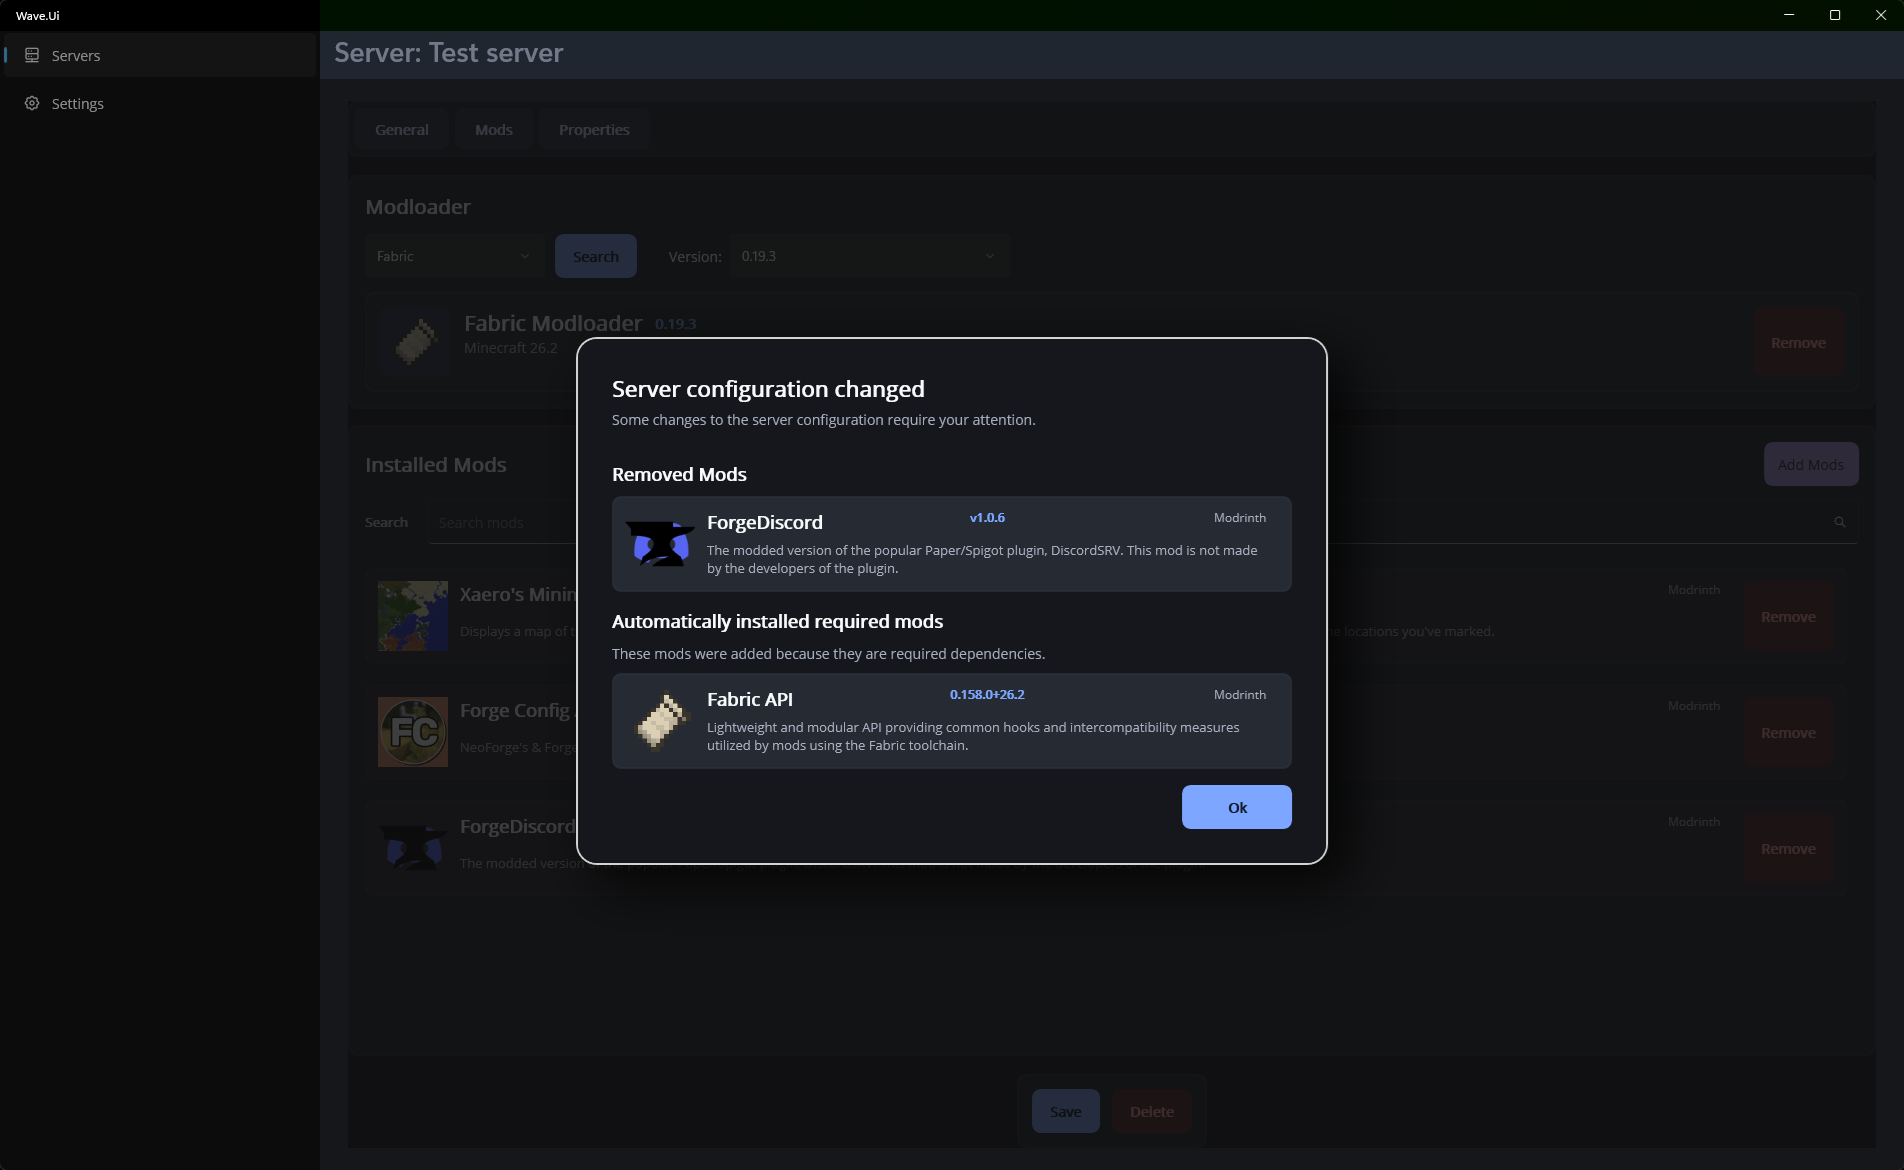
\includegraphics[width=\textwidth,height=0.72\textheight,keepaspectratio]{ChangeSummary.png}
  \caption{Summary of changes before updating a server.}
  \label{fig:guide-change-summary}
\end{figure}

\section{Starting and stopping}

The start action checks that the selected Java runtime exists and that another Wave server is not using the configured port. The application requests an automatic router mapping and starts the Java process only if this step succeeds. The Execution page shows the redirected output. Server commands can be entered while the session is active.

The normal stop action sends the server command that allows Minecraft to save its world, closes the process session and releases the temporary port mapping. Closing Wave Launcher also ends managed running sessions.

\begin{figure}[htbp]
  \centering
  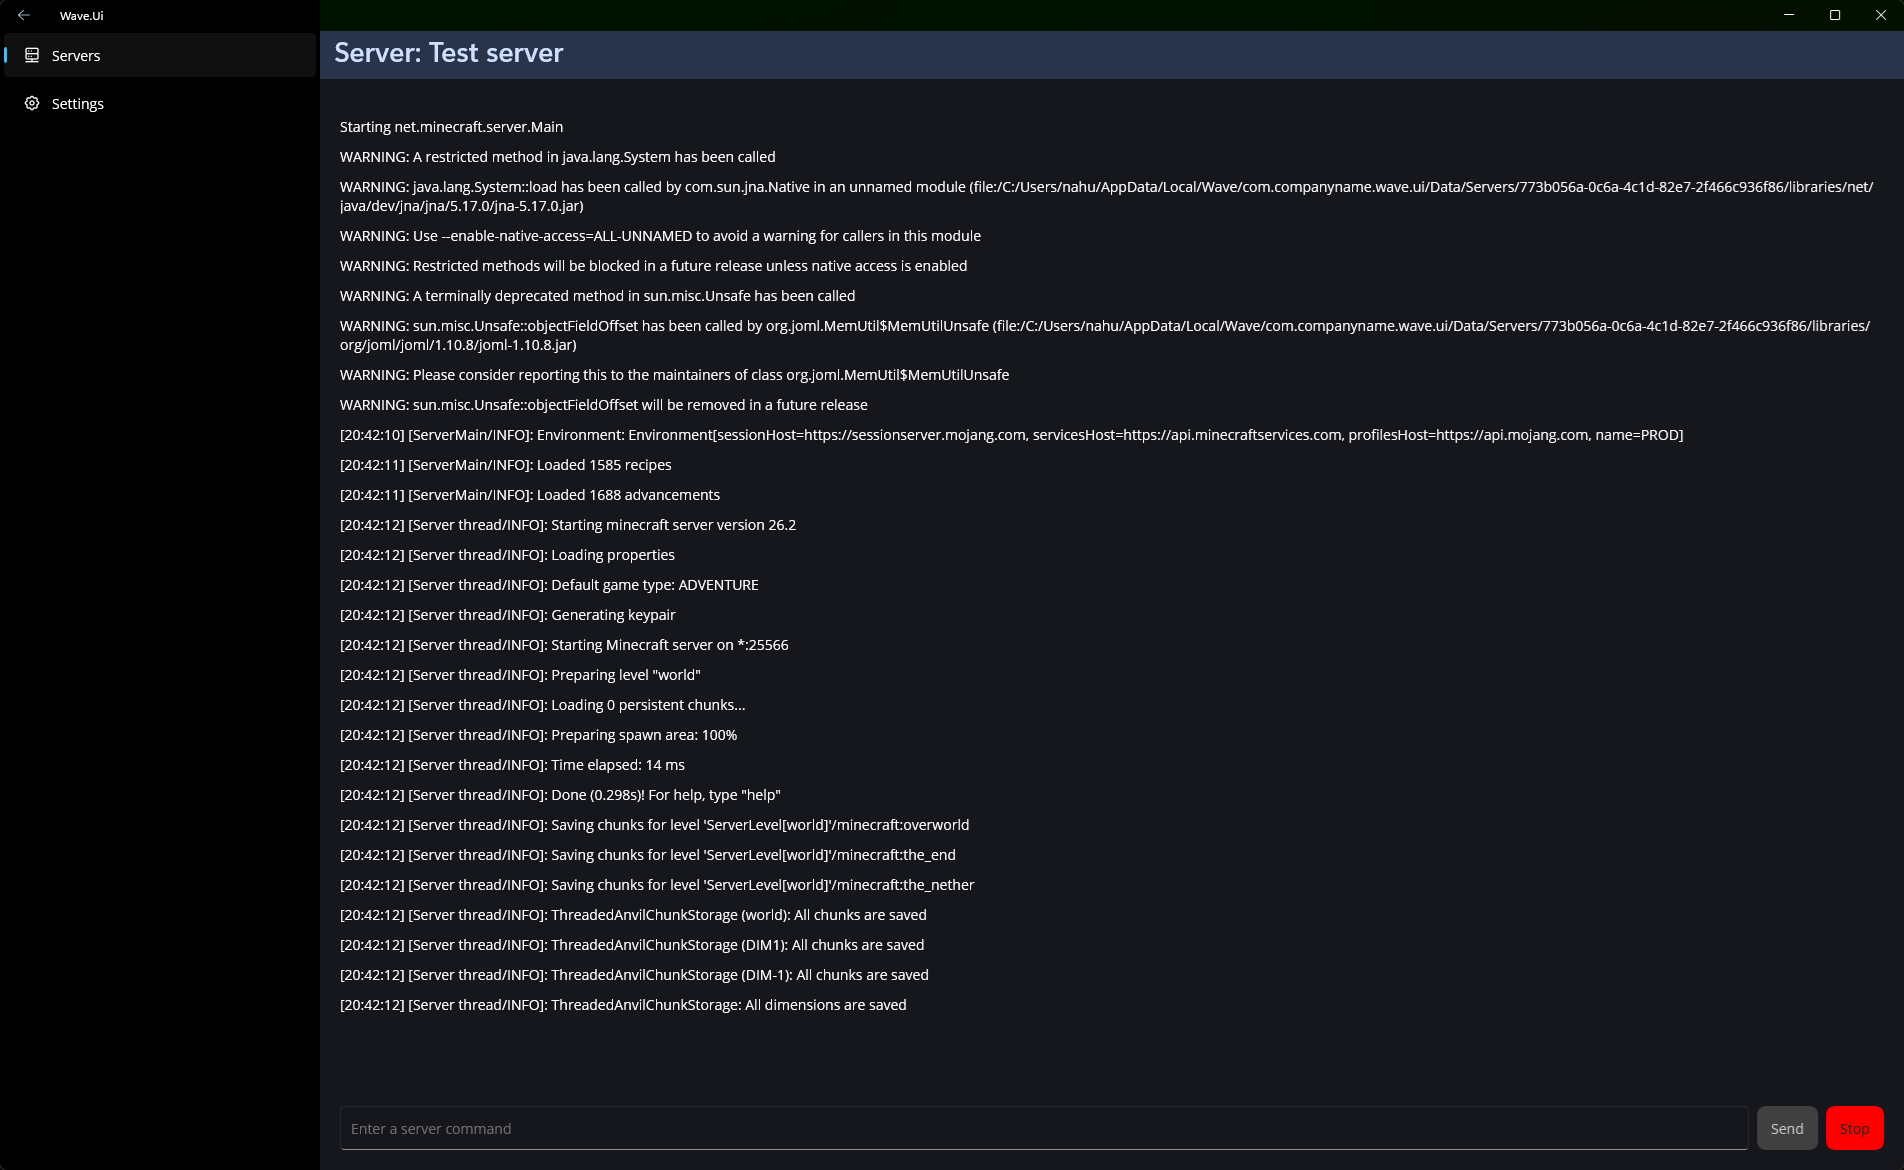
\includegraphics[width=\textwidth,height=0.72\textheight,keepaspectratio]{ServerExecutionPage.png}
  \caption{Execution console for a running server.}
  \label{fig:guide-server-execution}
\end{figure}

\section{Removing content}

Mods can be deselected through the server editor. Removing a loader also removes mods that depend on it. A Java installation must first be detached from every saved server before it can be uninstalled. Deleting a server removes its managed directory, including its world and configuration, so any world that must be retained should be copied before deletion.

\chapter{Repository structure}\label{ann:repository}

\begin{description}
  \item[\texttt{Wave.Domain}] Server, Minecraft, Java, mod, loader, device and pagination models.
  \item[\texttt{Wave.Application/In}] Operations consumed by view models.
  \item[\texttt{Wave.Application/Middle}] Contracts for managers used inside server workflows.
  \item[\texttt{Wave.Application/Out}] Repository, provider, process, platform, image and network ports.
  \item[\texttt{Wave.Infrastructure/In}] Implementations of the principal application use cases.
  \item[\texttt{Wave.Infrastructure/Middle}] Version, loader, mod, properties, EULA and path orchestration.
  \item[\texttt{Wave.Infrastructure/Out}] JSON persistence, external HTTP adapters, Java installers, Windows process execution and SharpOpenNat port mapping.
  \item[\texttt{Wave.Ui/Pages}] Pages, views and view models organized by content area.
  \item[\texttt{Wave.Ui/Views}] Reusable collections, forms, feedback and navigation controls.
  \item[\texttt{Wave.Ui/Resources}] Icons, images, fonts, colors and styles packaged by MAUI.
\end{description}
